% !TEX root = paper.tex
% =============================================================
% RAR -- Method Section v0
% Source-of-truth: project_context.md (binding constraints).
% Stage 3 of paper-writing skill. Draft 0 intro frozen 2026-07-09.
% Last updated: 2026-07-09
%
% Design spine (locked 2026-07-09):
%   per-flow historical compatibility -> soft routing
%   -> dual class paths -> calibration.
% Echoed in section opener and in each subsection.
%
% Conventions:
%   - KDD venue: integrated related work, colon-style subtitles,
%     no \smartparagraph, no em-dashes.
%   - Each design choice justified immediately ("we use X because Y").
%   - Headings are claims. Topic sentences assert claims.
%   - Cite prior work (autoencoders, knowledge distillation, etc.).
%   - Forward-reference evaluation subsections where relevant.
%   - Mechanism: SOFT routing. Do not describe RAR as assigning
%     each sample to a single head.
% =============================================================

\section{Method}\label{sec:method}

% Section opener: claim-first. Echoes the design spine so §1 and §3
% share the same thesis. We introduce the mechanism at the abstraction
% level; implementation follows in the subsections.

RAR's design follows a single line: per-flow historical compatibility, reconstruction-aware soft routing, dual class paths, and calibration. A reconstruction autoencoder over frozen traffic representations produces an old/new compatibility score for each flow. The same score weights the incremental objectives during training and integrates a frozen historical-class path with a trainable new-class path during inference. Logit calibration then maps the two outputs into a unified traffic-class space. The rest of this section defines each component and the assumptions that bound the mechanism.

\begin{figure*}[t]
\centering
% =============================================================
% RAR -- Figure 1: RAR architecture overview
% Label: fig:rar-architecture
% Used in: §3 Method (after the section opener).
% Format: input-style (no \documentclass). \input{} from paper.tex.
%   For standalone visual preview, wrap in
%     \documentclass[border=5pt]{standalone}
%     \usepackage{tikz} \usetikzlibrary{...}
%     \definecolor{ptblue}{HTML}{4477AA} ... (palette)
% Color palette: Paul Tol bright (matches figures/fig_*.tex).
% =============================================================

\begin{tikzpicture}[
    node distance=0.55cm and 0.7cm,
    box/.style={rectangle, draw, thick, rounded corners=3pt,
                minimum width=1.9cm, minimum height=0.75cm,
                font=\small\sffamily, align=center},
    raw/.style={box, fill=ptgrey!25},
    enc/.style={box, fill=ptblue!18},
    ae/.style={box, fill=ptcyan!18},
    prob/.style={box, fill=ptblue!10},
    hold/.style={box, fill=ptgreen!18},
    hnew/.style={box, fill=ptred!18},
    calib/.style={box, fill=ptblue!22},
    small/.style={font=\footnotesize\sffamily},
    smallit/.style={font=\footnotesize\sffamily\itshape},
    arrow/.style={-{Stealth[length=5pt]}, thick},
    arrowthin/.style={-{Stealth[length=4pt]}, thick, color=ptgrey},
]

% --- input ---
\node[raw] (in) {Raw\\input $x$};

% --- frozen encoder ---
\node[enc, right=of in] (enc) {Frozen\\encoder $f$};
\node[smallit, below=1pt of enc, color=ptblue!70!black] {frozen, shared};

% --- feature (fork point) ---
\node[small, right=0.55cm of enc] (feat) {$f(x)$};

% --- autoencoder branch (drops down then up) ---
\node[ae, below=1.0cm of feat] (ae) {Recon.\\autoencoder $g_\phi$};
\node[smallit, below=1pt of ae, color=ptcyan!70!black] {trained on old};

% --- sigmoid + threshold/tau ---
\node[prob, right=1.1cm of ae] (sig) {$\sigma((\theta - e)/\tau)$};
\node[prob, right=of sig] (gate) {log-space\\gate};
\node[smallit, above=1pt of sig, color=ptblue!70!black] {score $s_{\mathrm{old}}$};
\node[smallit, above=1pt of gate, color=ptblue!70!black] {$\log s \to \ell$};

% --- two heads ---
\node[hold, above=1.0cm of feat] (hold) {Old-knowledge\\head $h_{\mathrm{old}}$};
\node[smallit, above=1pt of hold, color=ptgreen!70!black] {frozen, inherited from base};
\node[hnew, right=2.4cm of hold] (hnew) {New-knowledge\\head $h_{\mathrm{new}}$};
\node[smallit, above=1pt of hnew, color=ptred!70!black] {adapter + MLP, trained};

% --- calibration ---
\node[calib, right=1.3cm of hnew] (calib) {Calibration\\$b_{\mathrm{old}}, c_{\mathrm{new}}, b_{\mathrm{new}}$};
\node[smallit, below=1pt of calib, color=ptblue!70!black] {3 scalar params};

% --- output ---
\node[raw, right=of calib] (out) {Joint\\logits};

% ============== arrows ==============
\draw[arrow] (in) -- (enc);
\draw[arrow] (enc) -- (feat);

% feature -> heads (fan-out)
\draw[arrow] (feat) -- (hold);
\draw[arrow] (feat) -- (hnew);

% feature -> autoencoder (down)
\draw[arrow] (feat) -- (ae);
% autoencoder -> sigmoid -> gate
\draw[arrow] (ae) -- (sig);
\draw[arrow] (sig) -- (gate);

% gate -> calibration (log-space routing signal feeds into combination)
\draw[arrow] (gate.east) -- ++(0.55cm,0) |- (calib.south);

% heads -> calibration
\draw[arrow] (hold) -- (calib);
\draw[arrow] (hnew) -- (calib);

% calibration -> output
\draw[arrow] (calib) -- (out);

% --- error term annotation ---
\node[small, color=ptgrey!80!black, above] at ($(ae)!0.5!(sig)$) {$e(x)$};

% --- legend hint ---
\node[small, color=ptgrey!70!black] at ($(in.south)+(0,-1.3cm)$)
    {frozen encoder (blue) $\cdot$ reconstruction (cyan) $\cdot$ old (green) $\cdot$ new (red)};

\end{tikzpicture}

\caption{RAR architecture overview.}
\label{fig:rar-architecture}
\Description{Architecture diagram of RAR. Each flow passes through a frozen ET-BERT encoder into feature vector f(x). Three parallel branches contain a frozen old-class path, a trainable new-class path with an adapter, and a reconstruction autoencoder that maps error through a sigmoid into routing scores. Log-space gating combines the two class-path outputs, followed by scalar calibration into joint logits.}
\end{figure*}

% -----------------------------------------------------------------
% 3.1 Problem formulation
% -----------------------------------------------------------------
\subsection{Problem Formulation}

Let $f: \mathcal{X} \to \mathbb{R}^d$ be a frozen encoder pre-trained on large-scale encrypted traffic data (ET-BERT~\cite{lin2022etbert}). At the base stage, we train a classifier $F_0$ on $K_0$ classes using $\mathcal{D}_0 = \{(x_i,y_i)\}_{i=1}^{N_0}$. At increment $t$, $K_t$ classes arrive with data $\mathcal{D}_t$, and a replay buffer $\mathcal{B}_{t-1}$ represents the classes seen before $t$. Let $K_{<t}=\sum_{j=0}^{t-1}K_j$ denote the number of previously learned classes. RAR freezes the complete preceding classifier $F_{t-1}$ as the old prediction path and learns a new-class head $h_t:\mathbb{R}^d\to\mathbb{R}^{K_t}$. For the single-increment setting, $F_{t-1}=F_0$ reduces to the frozen base classifier. Each flow is routed between $F_{t-1}$ and $h_t$ by a weight derived from reconstruction error. The following subsections define the reconstruction signal (\S\ref{sec:knowledge}), routing (\S\ref{sec:routing}), calibration (\S\ref{sec:calib}), and training procedure (\S\ref{sec:training}).

% -----------------------------------------------------------------
% 3.2 Per-flow reconstruction compatibility
% -----------------------------------------------------------------
\subsection{Per-Flow Reconstruction Compatibility}\label{sec:knowledge}

% Topic sentence 1: claim
RAR measures each flow's compatibility with the replay-derived historical-class manifold using a scalar routing score. This score is an operational weight, not a calibrated posterior probability or a hard assignment to one class group.

% Topic sentence 2: mechanism
We train a reconstruction autoencoder $g_\phi$ on frozen-encoder features of replayed old samples, so $g_\phi$ learns the manifold that the frozen encoder $f$ produces for old classes. The reconstruction error therefore tends to be small on old-class samples and large on new-class samples:
\begin{equation}\label{eq:recon}
e(x) = \frac{1}{d}\,\| g_\phi(f(x)) - f(x) \|_2^2.
\end{equation}
We compute the old 95th-percentile edge and new 5th-percentile edge on the replay and new reference sets, respectively, and set $\theta$ to their midpoint. The temperature $\tau$ is the pooled standard deviation of their errors, lower-bounded for numerical stability. We then convert the error to per-flow routing scores:
\begin{align}
s_{\mathrm{old}}(x) &= \sigma\!\left(\frac{\theta - e(x)}{\tau}\right),\label{eq:score-old}\\
s_{\mathrm{new}}(x) &= 1 - s_{\mathrm{old}}(x),\label{eq:score-new}
\end{align}
where $\tau$ controls the sharpness of the sigmoid. The fitted threshold and temperature are fixed after the pre-training stage; only $e(x)$ is computed per input at inference.

% Topic sentence 3: why reconstruction (design justification)
The score does not require a class label at inference: it measures compatibility between $f(x)$ and the feature manifold learned by $g_\phi$. Its fitting stage does use the known old/new split between replay and newly arriving reference samples. Reconstruction-based gating has previously been used to infer tasks and select experts~\cite{aljundi2017expertgate}; here, the score instead balances two class groups within a unified prediction space and weights the corresponding incremental-learning objectives. It complements output-based distillation (LwF~\cite{li2017lwf}, iCaRL~\cite{rebuffi2017icarl}) and stored-example replay (DER~\cite{yan2021der}).

% Topic sentence 4: empirical foundation
The empirical foundation for $s_{\mathrm{old}}$ is separability: across the six evaluated datasets, reconstruction error distinguishes old from new samples with mean AUC 0.894 (Figure~\ref{fig:e0-separability}). This result motivates evaluating the routing mechanism on the full benchmark; it does not imply perfect old/new identification.

\begin{figure*}[t]
\centering
% =============================================================
% RAR -- Figure 2: Reconstruction routing mechanism (detail)
% Label: fig:recon-routing
% Used in: Per-Flow Reconstruction Compatibility.
% Format: input-style (no \documentclass). \input{} from paper.tex.
%   For standalone visual preview, wrap in
%     \documentclass[border=5pt]{standalone}
%     \usepackage{tikz} \usetikzlibrary{...}
%     \definecolor{ptblue}{HTML}{4477AA} ... (palette)
% Color palette: Paul Tol bright (matches figures/fig_*.tex).
% =============================================================

\begin{tikzpicture}[
    node distance=0.6cm and 0.6cm,
    box/.style={rectangle, draw, thick, rounded corners=3pt,
                minimum width=1.7cm, minimum height=0.7cm,
                font=\small\sffamily, align=center},
    fbox/.style={box, fill=ptblue!15},
    ae/.style={box, fill=ptcyan!18},
    err/.style={circle, draw, thick, fill=ptgrey!20,
                minimum size=0.85cm, inner sep=1pt,
                font=\footnotesize\sffamily},
    sigbox/.style={box, fill=ptblue!18},
    taubox/.style={box, fill=ptblue!22},
    small/.style={font=\footnotesize\sffamily},
    smallit/.style={font=\footnotesize\sffamily\itshape},
    arrow/.style={-{Stealth[length=5pt]}, thick},
    arrowthin/.style={-{Stealth[length=4pt]}, thick, color=ptgrey},
]

% --- bounding dashed box (drawn first; nodes will sit on top) ---
\node[draw=ptcyan, very thick, dashed, rounded corners=6pt,
      minimum width=11.4cm, minimum height=3.6cm,
      label={[smallit, color=ptcyan!70!black]above left:Reconstruction routing}] (bound) {};

% --- feature input ---
\node[fbox, left=0.55cm of bound.west, anchor=east] (feat) {$f(x)$};

% --- autoencoder ---
\node[ae, right=0.9cm of feat] (ae) {Autoencoder\\$g_\phi$};

% --- error ---
\node[err, right=of ae] (err) {$e(x)$};

% --- sigmoid with fitted threshold + temperature ---
\node[sigbox, right=of err] (sig) {$\sigma((\theta - e) / \tau)$};
\node[smallit, below=1pt of sig, color=ptblue!70!black]
    {$s_{\mathrm{old}}(x)$};

% --- log-space gating ---
\node[taubox, right=of sig] (tau) {log-space\\gate};
\node[smallit, below=1pt of tau, color=ptblue!70!black]
    {$\ell + \log s$};

% --- output ---
\node[box, draw=ptcyan, thick, fill=ptcyan!8,
      right=0.9cm of tau] (out) {Gated\\logits};

% ============== arrows ==============
\draw[arrow] (feat) -- (ae);
\draw[arrow] (ae) -- (err);
\draw[arrow] (err) -- (sig);
\draw[arrow] (sig) -- (tau);
\draw[arrow] (tau) -- (out);

% --- external thin arrows showing f(x) also goes to heads ---
\draw[arrowthin] (feat.north) -- ++(0,0.5cm) node[above, small, color=ptgrey]
    {$\to$ heads $h_{\mathrm{old}}, h_{\mathrm{new}}$};

% --- tau + theta annotation ---
\node[small, color=ptblue!80!black, above=4pt of tau.north, anchor=center]
    {$(\theta, \tau)$ fitted on old/new errors};

% --- eqn under sigmoid ---
\node[small, color=ptgrey!70!black, align=center]
    at ($(ae.south)+(0,-0.85cm)$)
    {$\hat f(x) = g_\phi(f(x))$\\$e(x) = \mathrm{MSE}(\hat f(x), f(x))$};

\end{tikzpicture}

\caption{Reconstruction routing mechanism.}
\label{fig:recon-routing}
\Description{Detailed view of the reconstruction routing mechanism. Frozen encoder features pass through a feature reconstructor, producing reconstruction error via mean squared error. A fitted threshold and temperature map the error through a sigmoid into an old-sample score. The score is applied as an additive log-space gate to the dual-head logits before concatenation and calibration.}
\end{figure*}

\begin{figure}[t]
\centering
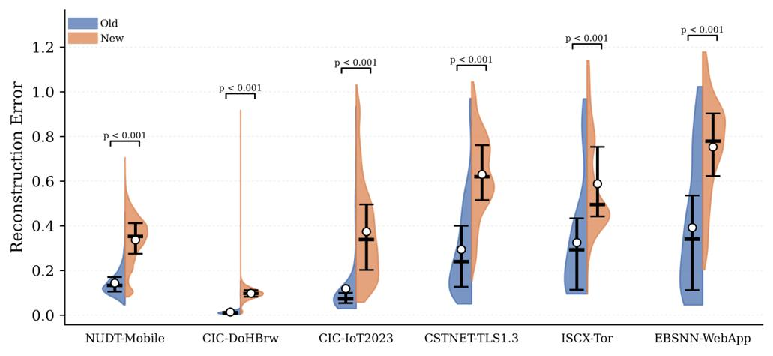
\includegraphics[width=\linewidth]{figures/fig_e0_separability.pdf}
\caption{Per-dataset reconstruction-error distributions (old vs.\ new).}
\label{fig:e0-separability}
\Description{Six-panel violin plot showing per-dataset distributions of reconstruction error for old and new samples. Blue violins represent old-class errors, orange violins represent new-class errors. All six datasets show statistically significant separation (p less than 0.001). Datasets: NUDT-Mobile, CIC-DoHBrw, CIC-IoT2023, CSTNET-TLS1.3, ISCX-Tor, EBSNN-WebApp.}
\end{figure}

% -----------------------------------------------------------------
% 3.3 Soft routing and dual class paths
% -----------------------------------------------------------------
\subsection{Soft Routing and Dual Class Paths}\label{sec:routing}

% Topic sentence 1: claim
RAR routes each flow through two class paths: the frozen preceding classifier $F_{t-1}$ and a trainable new-class head $h_t$ equipped with a lightweight adapter. Their outputs are weighted by $s_{\mathrm{old}}(x)$ and $s_{\mathrm{new}}(x)$ from Eqs.~\eqref{eq:score-old}--\eqref{eq:score-new}.

% Topic sentence 2: what each head does
In the first increment, the old path is the frozen base-stage classifier. In later increments, it is the complete recursively constructed RAR classifier from the preceding step and therefore covers all previously seen classes. The current new head is trained through a residual adapter and a LayerNorm+MLP pathway. The current encoder remains frozen.

% Topic sentence 3: soft routing mechanism
We apply the routing signal in log space. Let $\ell_{\mathrm{old}}(x) \in \mathbb{R}^{K_{<t}}$ and $\ell_{\mathrm{new}}(x) \in \mathbb{R}^{K_t}$ be the raw logit vectors from the two paths. The gated logits are computed by adding the log of each path's routing score:
\begin{align}
\tilde{\ell}_{\mathrm{old}}(x) &= \ell_{\mathrm{old}}(x) + \log s_{\mathrm{old}}(x),\label{eq:routing-old}\\
\tilde{\ell}_{\mathrm{new}}(x) &= \ell_{\mathrm{new}}(x) + \log s_{\mathrm{new}}(x).\label{eq:routing-new}
\end{align}
The two gated vectors are concatenated into a joint prediction over all $K_{<t} + K_t$ classes:
\begin{equation}\label{eq:concat}
\hat{y} = \mathrm{softmax}\bigl([\,\tilde{\ell}_{\mathrm{old}}(x)\;;\;\tilde{\ell}_{\mathrm{new}}(x)\,]\bigr).
\end{equation}
In softmax space, adding $\log s$ is equivalent to multiplying the head's class probabilities by $s$: the old-head probabilities are scaled by $s_{\mathrm{old}}(x)$ and the new-head probabilities by $s_{\mathrm{new}}(x)$, so both heads contribute to every prediction according to the flow's historical-class compatibility. As $\tau \to 0$ the sigmoid sharpens toward a step function and $s_{\mathrm{old}}$ approaches $0$ or $1$; as $\tau \to \infty$ the sigmoid flattens and both heads contribute near-equally. \S\ref{sec:eval-ablation-tau} reports the empirical trade-off.

% Topic sentence 4: why dual heads (design justification)
We separate old and new paths because standard head expansion makes their logits compete within one trainable decision space~\cite{rebuffi2017icarl,wu2019bic}. Under imbalanced replay, optimization can favor the newly arriving group. Freezing the preceding path prevents direct updates to its class-specific parameters, while the calibration step makes its logits comparable with those of the new head. Table~\ref{tab:ablation} measures the contribution of this separation.

% Topic sentence 5: soft vs hard
We use soft routing because hard assignment routes every sample to a single head and discards the second head's view entirely. On samples near the reconstruction-error decision boundary, the discarded head often holds the correct prediction. Soft routing keeps both views available and shifts their contribution with the input, so the calibration step is structurally necessary: the two heads cannot be averaged directly because they output logits over disjoint class subsets.

% -----------------------------------------------------------------
% 3.3 Logit calibration 
% -----------------------------------------------------------------
\subsection{Logit Calibration}\label{sec:calib}

% Topic sentence 1: claim
Each head outputs logits over its own class subset; a calibration layer removes the scale mismatch between the two paths before their logits are combined.

% Topic sentence 2: why calibration is needed
The two heads live on different class axes and may produce logits at different magnitudes. A naive concatenation would let the head with larger logits dominate Eq.~\eqref{eq:concat} regardless of the routing scores. Calibration equalizes the two heads' output scales on a held-out validation set before the logits are combined.

% Topic sentence 3: calibration mechanism
We learn three scalar parameters: a subtractive bias $b_{\mathrm{old}} \in \mathbb{R}$ on the old-path logits, a multiplicative scale $c_{\mathrm{new}} \in \mathbb{R}^+$, and an additive bias $b_{\mathrm{new}} \in \mathbb{R}$ on the new-head logits:
\begin{align}
\ell'_{\mathrm{old}} &= \tilde{\ell}_{\mathrm{old}} - b_{\mathrm{old}},\label{eq:calib-old}\\
\ell'_{\mathrm{new}} &= c_{\mathrm{new}} \cdot \tilde{\ell}_{\mathrm{new}} + b_{\mathrm{new}},\label{eq:calib-new}
\end{align}
where $\tilde{\ell}_{\mathrm{old}}, \tilde{\ell}_{\mathrm{new}}$ are the gated logits from Eqs.~\eqref{eq:routing-old}--\eqref{eq:routing-new}. The concatenation in Eq.~\eqref{eq:concat} then uses $[\ell'_{\mathrm{old}}; \ell'_{\mathrm{new}}]$. The three scalars are optimized with the new-class pathway during incremental training and then refined, with both prediction paths frozen, on a balanced calibration set formed from replayed old samples and held-out new samples.

% Topic sentence 4: what calibration does and does not do
Calibration does not change which classes the paths cover; it only adjusts their relative output scales. The classification decision remains a weighted combination in which the weights come from the reconstruction-derived routing score. Table~\ref{tab:ablation} reports its contribution.

% -----------------------------------------------------------------
% 3.4 Training objective and the temperature tau knob 
% -----------------------------------------------------------------
\subsection{Training Objective}\label{sec:training}

RAR training proceeds in three phases at each increment.

\paragraph{Phase 1: Fitting the reconstructor.}
We fit the reconstruction autoencoder $g_\phi$ on frozen-encoder features of replayed old samples by minimizing $\mathcal{L}_{\mathrm{recon}} = \frac{1}{|\mathcal{B}|}\sum_{x \in \mathcal{B}} \|g_\phi(f(x)) - f(x)\|_2^2$. We then estimate $\theta$ and $\tau$ from replayed-old and held-out-new errors as described in \S\ref{sec:knowledge}, and freeze $g_\phi$.

\paragraph{Phase 2: Incremental training.}
We freeze the preceding prediction path and optimize the adapter, new-class pathway, and calibration scalars with the following composite loss:
\begin{align}
\mathcal{L} &= \mathcal{L}_{\mathrm{CE}} + \alpha \mathcal{L}_{\mathrm{distill}} + \beta \mathcal{L}_{\mathrm{local}} + \gamma \mathcal{L}_{\mathrm{margin}} + \delta \mathcal{L}_{\mathrm{reg}},\label{eq:loss}\\[2pt]
\mathcal{L}_{\mathrm{distill}} &= \frac{1}{Z}\sum_{x \in \mathcal{B}} s_{\mathrm{old}}(x)\, D_{\mathrm{KL}}\bigl(F_{t-1}(x) \;\big\|\; \ell_{\mathrm{old}}(x)\bigr).\label{eq:distill}
\end{align}
Here $\ell_{\mathrm{old}}$ denotes the preceding path's logits after the trainable old-path bias, so the KL term anchors this adjustment to the frozen teacher output; the class-specific parameters of $F_{t-1}$ remain frozen. $\mathcal{L}_{\mathrm{CE}}$ is cross-entropy on the concatenated output over all classes; $\mathcal{L}_{\mathrm{local}}$ is cross-entropy restricted to the new head on new-class samples; $\mathcal{L}_{\mathrm{margin}}$ penalizes the old path for outscoring the correct new-class logit, weighted by $s_{\mathrm{new}}(x)$; and $\mathcal{L}_{\mathrm{reg}} = \|a(x) - f(x)\|_2^2$ regularizes the adapter shift from the frozen features. The replay buffer uses 1\% of the old training data in the main comparison; \S\ref{sec:eval-buffer} sweeps this ratio.

\paragraph{Phase 3: Calibration refinement.}
After incremental training, we freeze both prediction paths and refine $(b_{\mathrm{old}}, c_{\mathrm{new}}, b_{\mathrm{new}})$ on a balanced mixed calibration set by minimizing cross-entropy. The old portion is sampled from replay memory; the new portion comes from a fixed new-class validation partition that is excluded from final testing.

\subsection{Recursive Multi-step Update}\label{sec:multistep}
For sequential increments, RAR applies the same construction recursively. After increment $t$, the complete calibrated classifier $F_t$, including its earlier routing hierarchy, is frozen and used as the old path at increment $t+1$. The replay buffer is resampled from all classes seen through $t$, and a fresh reconstructor, threshold, temperature, adapter, and new-class head are fitted for the next class block. Consequently, the old output dimension grows from $\sum_{j=0}^{t-1}K_j$ to $\sum_{j=0}^{t}K_j$ without flattening the previous heads into a newly trainable shared classifier. This is the protocol used in the five-increment experiment in \S\ref{sec:eval-buffer}.

\paragraph{Algorithm.}
Algorithm~\ref{alg:rar} summarizes the full training and inference procedure.

\begin{algorithm}[t]
\SetAlgoNoLine
\KwIn{Frozen preceding classifier $F_{t-1}$; replay buffer $\mathcal{B}_{t-1}$; current data $\mathcal{D}_t$; reconstructor $g_\phi$; temperature $\tau$}
\KwOut{Incremental classifier $F$}
\For{each batch from $\mathcal{B} \cup \mathcal{D}_{\mathrm{new}}$}{
  \textbf{Feature extraction}\;
  \Indp
  $z \gets f(x)$ \quad (frozen, no gradient)\;
  \Indm
  \textbf{Reconstruction error}\;
  \Indp
  $e(x) = \frac{1}{d}\,\|g_\phi(z)-z\|_2^2$\;
  \Indm
  \textbf{Old/new routing score}\;
  \Indp
  $s_{\mathrm{old}}
  = \sigma\!\left(\frac{\theta-e(x)}{\tau}\right)$\;
  $s_{\mathrm{new}}
  = 1-s_{\mathrm{old}}$\;
  \Indm
  \textbf{Dual-head routing (log-space)}\;
  \Indp
  $\tilde{\ell}_{\mathrm{old}}
  = \ell_{\mathrm{old}}
  +\log s_{\mathrm{old}}$\;

  $\tilde{\ell}_{\mathrm{new}}
  = \ell_{\mathrm{new}}
  +\log s_{\mathrm{new}}$\;

  $\hat{y}
  =\mathrm{softmax}
  ([\tilde{\ell}_{\mathrm{old}};
  \tilde{\ell}_{\mathrm{new}}])$\;
  \Indm

  \textbf{Training objective}\;
  \Indp
  $\mathcal{L}
  =
  \mathcal{L}_{\mathrm{CE}}
  +\alpha\mathcal{L}_{\mathrm{distill}}
  +\beta\mathcal{L}_{\mathrm{local}}
  +\gamma\mathcal{L}_{\mathrm{margin}}
  +\delta\mathcal{L}_{\mathrm{reg}}$\;
  \Indm
}
\textbf{Post-hoc calibration}\;
\Indp
$\ell'_{\mathrm{old}}
=\tilde{\ell}_{\mathrm{old}}-b_{\mathrm{old}}$\;

$\ell'_{\mathrm{new}}
=c_{\mathrm{new}}\cdot\tilde{\ell}_{\mathrm{new}}+b_{\mathrm{new}}$\;

Refine $(b_{\mathrm{old}}, c_{\mathrm{new}}, b_{\mathrm{new}})$ on the mixed calibration set (paths frozen)\;
\Indm
\Return $F$
\caption{Reconstruction-Aware Routing (RAR)}
\label{alg:rar}
\end{algorithm}

% Topic sentence 5: the tau knob
The temperature $\tau$ trades routing determinism against path fusion. In the implementation it is estimated from the pooled reconstruction-error spread; \S\ref{sec:eval-ablation-tau} additionally reports a controlled sensitivity sweep. Lowering $\tau$ makes the routing weights more discrete, but does not by itself reduce computation because both paths are still evaluated.

% -----------------------------------------------------------------
% 3.5 Assumptions and failure modes 
% -----------------------------------------------------------------
\subsection{Applicability and Assumptions}\label{sec:assumptions}

RAR is designed under two key assumptions that define its applicability.

First, replay memory should provide representative coverage of previously learned classes. If replay samples fail to capture the historical-class distribution, the reconstructor may learn an incomplete historical manifold, leading to inaccurate routing scores. \S\ref{sec:eval-buffer} evaluates different replay buffer sizes and shows that RAR remains robust even under a memory ratio of 0.005.

Second, reconstruction error should exhibit sufficient separability between old and emerging knowledge. When old and new classes have highly similar feature representations, reconstruction errors may overlap, reducing the reliability of the compatibility score. Figure~\ref{fig:e0-separability} shows the observed separation across the six evaluated datasets.

These assumptions characterize the applicability of RAR rather than strict limitations. RAR is most effective when replay samples preserve representative historical-class coverage and when old and emerging classes exhibit distinguishable representation patterns.
